\section{System}

    Ein System ist ein Operator der ein Signal ändert.
    \subsection{Systemklassifikationen}
        %SISO = Single Input Single Output
        %MIMO = .....
        \textbf{Lineares System:}
                Ein System heisst linear, falls gilt: 
                \[\Sigma (\alpha \cdot u_1 + \beta \cdot u_2) = \alpha \cdot \Sigma (u_1) + \beta \cdot \Sigma(u_2)\]   
            \begin{center}
            \begin{tabular}{ c c }
                \textbf{Linear:} & \textbf{Nichtlinear:} \\ 
                \hline
                $ y(t) = \frac{d}{dt}u(t)$& $ y(t) = \alpha \cdot u(t) + \beta $ \\  
                \hline
                $y(t) = \int_0^t u(\tau)d\tau$ & $ y(t) = \sin{\left(u(t)\right)}$ \\
                \hline
                $y(t) = \alpha\cdot u(t)$ & $y(t) = \sqrt{u(t)}$
            \end{tabular}
            \end{center}
        \textbf{Kausal/Akausal:} Ein kausales System hängt nicht von Eingängen in der Zukunft ab.
        
        $\rightarrow$ Alle physikalische Systeme sind kausal.
        
        \begin{center}
        \begin{tabular}{ c c }
            \textbf{Kausal:} & \textbf{Akausal:} \\ 
                \hline
                $ y(t) = u(t -\tau)$ 
                   $ \forall\tau \geq 0 $ & $y(t) = u(t+5) $ \\  
                \hline
                $y(t) = \int_0^{-\infty} u(\tau)d\tau$ & $ y(t) = \int_{-\infty}^{t+1}u(\tau) d\tau $
        \end{tabular}
        \end{center}
    \textbf{Dynamisch/Statisch:}
        Der Ausgang bei \textbf{Statischen} Systemen zur Zeit $t^*$ hängt nur vom Eingang zur Zeit $t^*$ ab.
        
        \begin{center}
        \begin{tabular}{ c c }
            \textbf{Dynamisch:} & \textbf{Statisch:} \\ 
                \hline
                $ y(t) = u(t -\tau)$ 
                   $ \forall\tau \neq 0 $ & $y(t) = \sqrt{u(t)} $ \\ 
                \hline
                $y(t) = \int_0^{t} u(t-\tau)d\tau$ & $ y(t) = 3\cdot u(t) $
        \end{tabular}
        \end{center}
    \textbf{Zeitvariant/Zeitinvariant:} Zeitvariante Systeme geben bei gleichen            Eingängen zu unterschiedlichen Zeitpunkten und gleicher Anfangsbedingungen     unterschiedliche    
    Ausgänge.
         \begin{center}
            \begin{tabular}{ c c }
                \textbf{Zeitinvariant:} & \textbf{Zeitvariant:} \\ 
                    \hline
                    $ y(t) = 3 \cdot u(t)$ & $y(t) = \sin{\left(t\right)} \cdot u(t) $ \\ 
                    \hline
                    $y(t) = \frac{d}{dt}u(t)$ & $ y(t) = u(t) + t $
            \end{tabular}
        \end{center}
    Transfer Functions $\Sigma(s)$ sind immer linear und zeitinvariant.
    
    \subsection{Steuerung/Regelung/Vorsteuerung}
        \textbf{Feed forward/Open Loop:} (Steuerung) Ausgangsgrösse y wird schnell erreicht aber kann bei kleinen Störungen schon nicht mehr exakt reguliert werden, da die Ausgangsgrösse nicht mit der Führungsgrösse r verglichen wird.
        
        \textbf{Feedback/Closed Loop:} (Regelung) Man fängt 'bei Null' an und schaut was die Ausgangsgrösse y ist. Diese wird auf Führungsgrösse r zurückgeführt um Fehler e zu bilden, der durch den Controller zu einer Regelung der Strecke führt. Gewünschte Ausgangsgrösse kann auch bei Störungen erreicht werden.
        
        \textbf{Vorsteuerung:} Ziel der Vorsteuerung ist es, das System durch Vorwissen des Verhalten der Regelstrecke in die Umgebung des gewünschten Operationspunktes zu steuern. Der Fehler der durch die Vorsteuerung versuracht wird, wird durch die Regelung korrigiert
        
        \subsubsection{Bsp}
            \begin{center}
                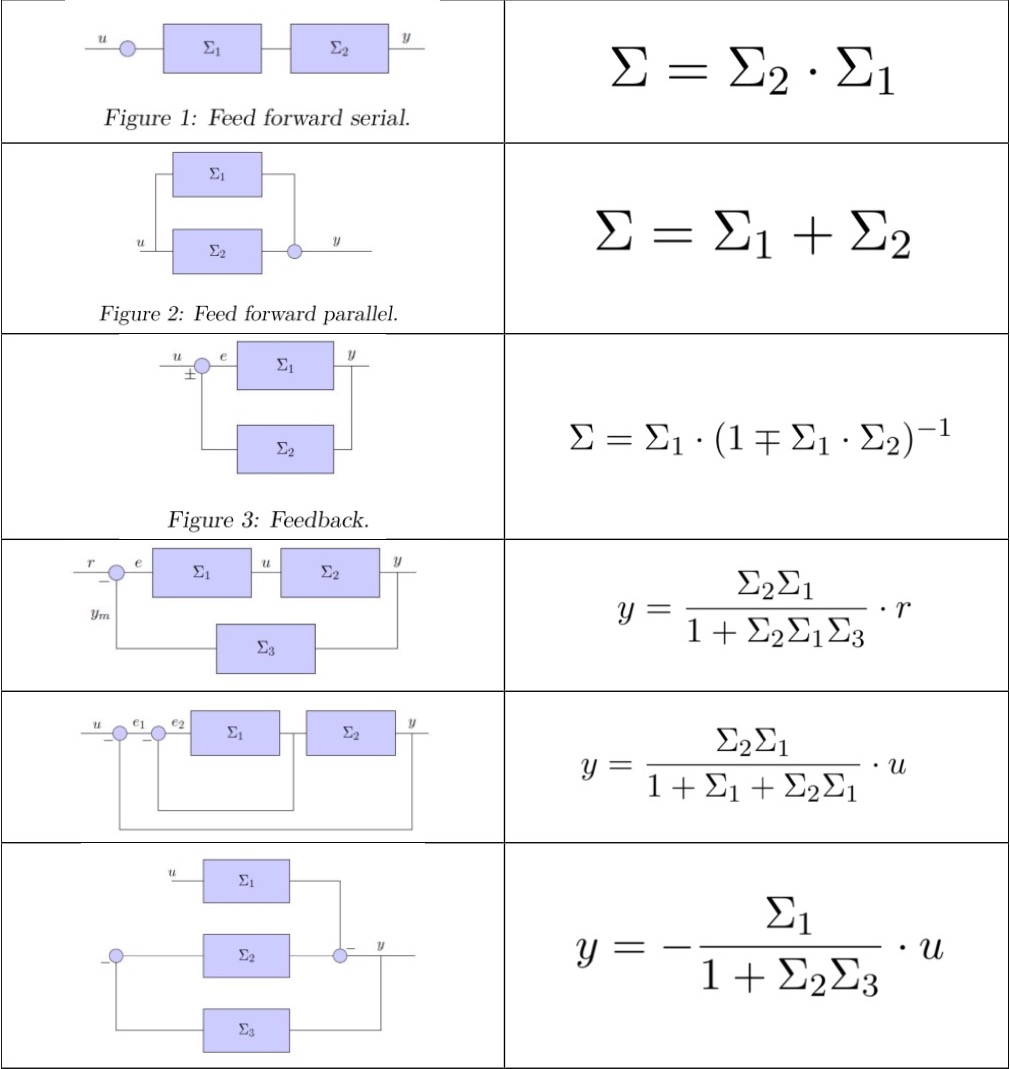
\includegraphics[width=0.75\linewidth]{01/01_signalfluesse.jpg}
            \end{center}
